
\documentclass[a4paper]{book}
\title{Reti Logiche made Friendly}
\author{Matteo Sabella 218614}
\usepackage{graphicx}
\usepackage{wrapfig}
\usepackage[export]{adjustbox}
\usepackage{titlesec}
\usepackage{listings}
\usepackage{xcolor}
\usepackage{colortbl}
\graphicspath{{images/}}
\usepackage{wrapfig}
\definecolor{backcolour}{rgb}{0.95,0.95,0.92}
\definecolor{codegreen}{rgb}{0.4, 0.521, 0.454}
\definecolor{codegray}{rgb}{0.5,0.5,0.5}
\definecolor{codepurple}{rgb}{0.850, 0.203, 0.419}



\lstdefinestyle{mystyle}{
    backgroundcolor=\color{backcolour},   
    commentstyle=\color{codegreen},
    keywordstyle=\color{codepurple},
    numberstyle=\tiny\color{codegray},
    stringstyle=\color{codepurple},
    basicstyle=\ttfamily\footnotesize,
    breakatwhitespace=false,         
    breaklines=true,                 
    captionpos=b,                    
    keepspaces=true,                 
    numbers=left,                    
    numbersep=5pt,                  
    showspaces=false,                
    showstringspaces=false,
    showtabs=false,                  
    tabsize=2
}

\lstset{style=mystyle}





\begin{document}

\maketitle

%Al mio fedele compagno di avventure, che mi piaceva girare a letto come un flip flop e che mi ha consentito di mantenere la fede.%

\chapter{Da analogico a digitale}
Nell'era pre digitale i segnali erano analogici, ossia il loro valore spaziava su una gamma potenzialmente infinita di valori, in qualche forma proporzionali ad una qualche grandezza di interesse.
Ciò poneva di fronte ad un problema, quello delle interferenze e dei disturbi di segnale, che potevano distorcere o rendere impossibile la lettura del messaggio trasportato dal segnale in questione.
Si è perciò deciso di ricorrere al mezzo digitale, ossia un particolare modo di rappresentare le informazioni.
Ogni segnale può assumere solo due possibili valori(da qui denominato segnale binario), che si distinguono grazie ad un confine detto soglia che li separa.
Al di sotto di tale soglia il segnale ha ovunque lo stesso valore, così come al di sopra, ma tra una parte della soglia e l'altra, lì il valore cambia.
Tanto più il segnale è lontano dalla soglia tanto più esso può subire distorsioni senza che il messaggio venga all'arrivo compromesso.
Tale sistema però pone uno svantaggio, ossia l'impossibilità di comunicare un vasto numero di messaggi.
Per risolvere questo inconveniente intrinseco del modo di comunicare si ricorre a più sorgenti di segnali, così che invece che avere solo 2 possibili valori, il messaggio costituito da n segnali avrà \(2^n\) possibili significati o sfumature.
Questo non presenta un problema eccessivamente complicato da gestire, infatti essendo logaritmica la relazione tra il numero di rappresentazioni desiderate e il numero di segnali, il numero di segnali necessario cresce lentamente rispetto al numero rappresentazioni che si desiderano ! 

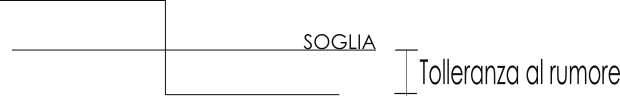
\includegraphics[width=\textwidth]{SchemaDigitale}

\newpage
\section*{Tecnologie di implementazione}

Successivamente alla descrizione della rete logica, c'è la sua realizzazione che produce un circuito integrato. 
Questa implementazione può avvenire in modi differenti :
\\(Si tenga presente che il prezzo per la realizzazione di un circuito dipende dalla sua estensione in superficie)

\begin{itemize}
\item
	\textbf{Full custom}\\
Un processo che permette di avere il controllo su ogni singolo transistore e collegamento. Fornisce un prodotto molto piccolo, con grandi prestazion ma è molto costoso. 
\item
	\textbf{Standard Cell / ASIC}\\
Utilizza delle celle già realizzate che vengono unite in base alle necessità per realizzare il circuito integrato.
E' meno costoso del progetto full custom e fornisce alte prestazioni.
\item
	\textbf{FPGA}\\
Sono schede già pronte su cui l'utente può programmare e configurarne i componenti per ottenere il circuito che vuole.
\item
	\textbf{Embedded Software}\\
Microprocessori senza controllo dei collegamenti e con logica programmabile.
\end{itemize}

\chapter{Circuiti combinatori}
\section{Operatori}
\subsection{OPERATORI SEMPLICI}
Gli operatori basilari che vengono utilizzati per la costruzione di reti logiche sono i seguenti:\\
\subsubsection*{AND}
\begin{wrapfigure}{r}{0.10\textwidth}
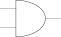
\includegraphics{AndPrecisa}
\end{wrapfigure}
L'operatore AND prende in input  due segnali e restituisce 1 se e solo se entrambi sono 1, altrimenti restituisce 0.
\\ Si rappresenta come : \(x*y\)\\


\subsubsection*{OR}
\begin{wrapfigure}{r}{0.10\textwidth}
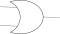
\includegraphics{OrGate}
\end{wrapfigure}
L'operatore OR prende in input due segnali e restituisce 1 se almeno uno dei due è 1, altrimenti restituisce 0.
\\ Si rappresenta come : \(x+y\)\\
\subsubsection*{NOT}
\begin{wrapfigure}{r}{0.10\textwidth}
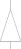
\includegraphics{NotGate}
\end{wrapfigure}
L'operatore NOT prende in input un solo segnali e restituisce 1 se il segnale è 0 e 0 se l'input è 1.
\\ Si rappresenta come : \(x'\)

\newpage
\subsection{OPERATORI COMPLESSI}
Gli operatori che vediamo di seguito possono essere considerati come operatori "complessi" ossia costituiti da elementi più semplici.
\begin{wrapfigure}{r}{0.10\textwidth}
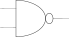
\includegraphics{NandGate}
\end{wrapfigure}
\subsubsection*{NAND}
L'operatore NAND è costituito da un operatore AND seguito da un NOT.
\begin{wrapfigure}{r}{0,10\textwidth}
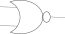
\includegraphics{NorGate}
\end{wrapfigure}
\subsubsection*{NOR}

L'operatore NOR è costituito da un operatore OR seguito da un NOT.

\subsubsection*{EXOR}
L'operatore EXOR è anche detto OR esclusivo, questo perchè restituisce 1 se e solo se i due segnali in ingresso sono diversi tra loro.
\subsubsection*{EXNOR}
L'operatore EXNOR è anche detto OR inclusivo perchè restituisce 1 se e solo se i due segnali in ingresso sono uguali tra loro.

\newpage
\section{Algebra di boole}
Le operazioni svolte dagli operatori appena visti godono di proprietà che vanno sotto il nome di algebra di Boole.\\ (Ognuna di esse è dimostrabile tramite induzione completa, ossia verificando totalmente la veridicità delle implicazioni tramite tabelle di verità).

\subsection*{Identità}

\(x+0=x \) \\
\(x*1=x \)

\subsection*{Complementazione}

\(x+x'=1 \) \\
\(x*x'=0 \)

\subsection*{Proprietà commutativa}

\(x+y=y*x \) \\
\(x*y=y*x \) 

\subsection*{Proprietà distributiva}

\( x*(y+z)=(x*y)+(x*z)  \) \\
\( x+(y*z)=(x+y)*(x+z)  \)

\subsection*{Proprietà associativa}

\(x+(y+z)=(x+y)+z \) \\
\(x*(y*z)=(x*y)*z \) 

\subsection*{Leggi di De Morgan}

Consentono di trasformare delle funzioni in cui compaiono OR in funzioni equivalenti che usano delle AND.\\
\( (x+y)' = x' * y' \) \hspace{3cm} \( (x'+y')' = x*y\) \\
\( (x*y)' = x' + y' \) \hspace{3cm} \( (x'*y')'= x+y\)
\\
\\
\textbf{Tip}:\\ Un modo utile per ricordarsele è che per passare da un operatore ad un altro , si cambia l'operatore e si "raccoglie" un not.

\newpage
\section{Teorema Di Shennon}
Nel processo di ricerca di un'espressione logica che impieghi gli operatori che ora conosciamo, torna utilissimo il teorema di Shennon.
Per ogni funzione logica del tipo\\\\ \( f({x_1},{x_2},{x_3},...,{x_n}) \)\\\\vale la seguente uguaglianza.\\\\ \(f({x_1},{x_2},{x_3},...,{x_n})=a*f(1,{x_2},{x_3},...,{x_n})+a'*f(0,{x_2},{x_3},...,{x_n})\)\\\\
Questa uguaglianza è valida perchè se a valesse 1, allora la parte di destra dell'OR sarà un AND con sicuramente valore 0 e quindi verrà come risultato il valore della prima espressione, altrimenti se a fosse 0 varrebbe lo stesso discorso ma al contrario.
\subsection{Forme canoniche}
Procedendo iterando questo teorema sui pezzi di funzioni rimanenti si può arrivare ad un'espansione nella seguente forma:
\\\\
\(f({x_1},{x_2},{x_3},...,{x_n})=a*f(1,{x_2},{x_3},...,{x_n})+a'*f(0,{x_2},{x_3},...,{x_n})\)
\\\\
Ciò può essere iterato fino ad ottenere una funzione costituita da sole somme e prodotti logici senza alcuna funzione all'interno di essa !\\
La forma così espansa della funzione logica iniziale è univoca per una data funzione e vien detta \textbf{forma canonica}\\\\
La forma canonica rende possibile esprimere ogni funzione tramite gli operatori logici di base.
Addirittura permette di esprimere ogni funzione logica anche solo con 'utilizzo di 2 su 3 operatori di base, perchè OR e AND possono essere esclusi mutuamente in quanto unendo uno dei due con una not seguendo le leggi di de morgan poss ottenere il comportamento dell'altra.
Esiste anche una seconda forma canonica che usa OR ed AND in modo diverso permettendo di ottenere la stessa funzione in un'altra forma.

\newpage

\chapter{Semplificazione di funzioni logiche}
Introduciamo ora alcune definizioni:\\
\begin{itemize}
\item\textbf{Livelli}
Il numero di livelli di un circuito è il numero massimo di porte logiche che possono essere attraversate all'interno di esso dall'ingresso all'uscita.
(non si tiene conto dei NOT)
\item\textbf{Letterale}
Ogni variabile che sia affermata o negata.\\
\item\textbf{Minterm}
Prodotto in cui ogni variabile compare una volta come letterale.\\ Esso è 1 per una e una sola combinazione di letterali.\\
\item\textbf{Maxterm}
Somma in cui ogni variabile compare una volta come letterale.\\ Esso è 0 per una e una sola combinazione di letterali.\\
\item\textbf{Implicante}
f è implicante di g se e solo se quando f è 1 allora g è 1.
\vspace{\baselineskip}
\\ Si dice \textbf{implicante primo} ogni implicante che non è possibile racchiudere in uno più grande.
Essi possono essere \textbf{ridondanti} nel caso in cui coprano zone coperte da altri implicanti primi mentre altri sono invece \textbf{essenziali} perchè sono gli unici a coprire quelle zone.

\vspace{\baselineskip}
\newpage
Ogni minterm è un implicante della propria f, l'unico problema è che ognuno di essi rappresenta "pochi uni".\\\break
\end{itemize}

La funzione logica sarà data dall' \textbf{OR} degli implicanti, ma quali cerco ?
\vspace{\baselineskip}

Partendo dalla tabella della verità si possono trovare i minterm della funzione.\\Questi poi possono essere compattati utilizzando le proprietà dell'algebra di Boole (torna molto utile l'adiacenza logica).

L'adiacenza logica in particolare si può utilizzare solo quando, dati minterm composti da L letterali, L-1 letterali restano immutati ed uno solo cambia.

Per trovare implicanti che non siano minterm è utile utilizzare la \textbf{notazione Gray}.\\
Chiamiamo \textbf{term} gli implicanti che non sono minterm !.\\
Essa consiste nel fare tabelle di verità in cui tra ogni riga e la sua successiva c'è solamente una variabile a variare, così da poter eventualmente fare dei raccoglimenti sfruttando l'algebra di Boole.


Non garantisce tuttavia un modo perfetto per trovare i minterm con facilità perchè permette di muoversi in una sola dimensione.

\vspace{\baselineskip}

Nel caso funzioni con più di due variabili è necessario cercare gli implicanti utilizzando altri modi per rappresentare le tabelle di verità così da far risaltare meglio le adiacenze tra i vari minterm.\\
\vspace{\baselineskip}
Qui entra in gioco \textbf{la mappa di Karnough}
\vspace{\baselineskip}
\begin{tabular}{|c|c|c|c|c|}
\hline
a$\backslash$ bc & 00 & 01 & 11 & 10 \\
\hline
0              & *  & *  & *  & *  \\
\hline
1              & *  & *  & *  & *  \\
\hline
\end{tabular}
\vspace{\baselineskip}
L'unica adiacenza non immediata è quella tra prima ed ultima colonna e tra prima ed ultima riga !
Nella prima riga partendo dall'alto verranno messe in notazione Gray tutte le possibili combinazioni che la variabile bc può assumere.
Nella prima colonna invece tutte le combinazioni (in questo caso solo essere raccolto e che finisce nella parentesi in OR con il suo negato e quindi come risultato da 1 
"scomparendo". 

L'unica adiacenza non immediata è quella tra prima ed ultima colonna e tra prima ed ultima riga !

Trovati i term, prima di fermarci, dobbiamo minimizzare il più possibile gli elementi in OR tra loro.
Questo è possibile trovando un certo tipo di implicanti, gli \textbf{implicanti primi}.
Ossia gli implicanti che non sono contenuti in nessun altro implicante più grande.
\newpage
\section{Insiemi di operatori completi ed uso delle porte logiche}

\section{Mappe a 4,5 e 6 variabili}
Le mappe saranno fatte esattamente come fatto fino a qui con la differenza che aumenterà la loro dimensione in modo esponenziale.
Infatti per ogni variabile che aggiungiamo le possibili combinazioni degli ingressi vengono raddoppiate !
(Continueremo ad usare il codice Gray)
Avremo quindi per mappe a 4 variabili delle mappe quadrate i cui minterm saranno composti da 4 letterali.

Nel caso di mappe da 4 variabili, ora esse saranno quadrate perchè avrò combinazioni di due ingressi sia sulle righe che sulle colonne.

Nel processo di sintetizzazione di una funzione quando si hanno a disposizione più scelte bisogna scegliere quella con minori implicanti, così che il circuito corrispondente poi abbia misure più contenute.
Per arrivare a ciò è utile cercare di minimizzare le sovrapposizioni.





\section{Altri metodi per sintetizzare circuiti}
\section{Minimizzazione congiunta}
\newpage	
\chapter{Circuiti Combinatori Fondamentali}

Di seguito vengono rappresentati, analizzati e spiegati alcuni circuiti combinatori che sono ritenuti fondamentali in quanto compaiono molto spesso e per cui è bene ricordarsi come sono fatti per non perdere tempo.
\section{Multiplexer}
In generale un multiplexer è una funzione logica che tramite un criterio prende delle variabili in entrata e ne restituisce una di esse.
\subsection{Da 2 a 1}
Ora prendiamo in esame il più elementare tra i multiplexer, ovvero quello che fa una decisione tra due varibili in ingresso.
Questo è il più elementare perchè altrimenti avrei una variabile in ingresso ed una in uscita e ciò non è un vera scelta.

Partiamo dalla tabella di verità scritta con il codice Gray e cerchiamone gli implicanti primi.
Partiamo da qui perchè è il punto principale per impostare come funzionerà il nostro multiplexer.\\

\begin{tabular}{|c|c|c|c|c|}
\hline
S-AB & 00 & 01 & 11 & 10 \\ \hline
0 &    0  &  0 & \cellcolor{yellow}1  & \cellcolor{yellow}1  \\ \hline  
1 &    0  &  \cellcolor{yellow}1 & \cellcolor{yellow}1  & 0  \\
\hline
\end{tabular}\break


Gli implicanti primi sono: SB, AB, S'A.
Quindi la nostra funzione può essere scritta come segue:
\( f=\) SB+S'A

Cerchiamo di capire cosa ci sta dicendo questa funzione.
Premettiamo che la convenzione che S=0 selezioni A mentre S=1 selezioni B è nostra scelta, con alcune differenze può avvenire benissimo anche il caso in cui S=0 selezioni B mentre S=1 selezioni A.

Prendendo in esame uno solo delle AND, queste ci dicono che nel caso in cui S sia 0 SICURAMENTE quel termine sarà del tutto irrilevante nel passaggio successivo costituito da un OR.
Perciò verrà selezionato ESCLUSIVAMENTE l'operazione AND che ha S=1.
Poi l'essere 0 o 1 dell'altro operando determinerà l'uscita esattamente di quel valore.



\begin{wrapfigure}{r}{0,1\textwidth}
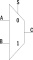
\includegraphics{Multiplexer21}
\end{wrapfigure}


Il multiplexer 2 a 1 si rappresenta con un questo simbolo circuitale:
In cui i numeri indicano per quale valore di S venga selezionata la corrispondente entrata.

\begin{figure}
\centering
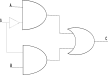
\includegraphics{Multiplexer21Circuito}
\caption{schema circuitale di un Multiplexer 2 a 1}
\end{figure}


\subsection{Da 4 a 1}

Alla luce di quello che abbiamo appena letto riguardo al multiplexer 2 a 1 possiamo immaginare come realizzare questa versione più in grande.

Posso utilizzare due multiplexer 2 a 1 per ottenere due output e poi questi ultimi metterli all'interno di un ulteriore multiplexer 2 a 1 così da ottenere un solo risultato in uscita.

\(S_01 \) si occuperà di scremare tra A e B mentre \(S_02 \) scremerà tra C e D.


\section{Odd Function}

E' una funzione che vale 1 SOLO se il numero di ingressi ad 1 è dispari.\\
Iniziamo sviluppando la tabella di Karnaugh.\\

\vspace{\baselineskip}

\begin{tabular}{|c|c|c|c|c|}
\hline
a$\backslash$ bc & 00 & 01 & 11 & 10 \\
\hline
0              & 0  &  \cellcolor{yellow}1 & 0  & \cellcolor{yellow}1  \\
\hline
1              & \cellcolor{yellow}1  &  0 & \cellcolor{yellow}1  & 0  \\
\hline
\end{tabular}
\vspace{\baselineskip}\\
Purtroppo i term in questo caso coincidono con i minterm della tabella di karnaugh e sono : ab'c' , a'b'c , abc , a'bc.\\
Quindi la funzione logica dell'odd counter è :
\\\\
\(f=\)ab'c'+a'b'c+abc+a'bc'
\\\\
Possiamo ora procedere a raggruppare eventuali term sfruttando l'adiacenza logica.
\\
\(f=\)b'(ac'+a'c)+b(ac+a'c') che possiamo ulteriormente compattare riconoscendo in ac'+a'c l'operatore booleano XOR e in ac+a'c l'operatore booleano XNOR.




\section{Conta Uni}

Lo scopo di questo circuito è dire in uscita quanti degli ingressi sono a 1. Nel nostro caso ci saranno 3 ingressi, quindi il numero in uscita potrà variare da 0 a 3 ossia da 00 a 11 in binario.


Chiamando gli ingressi a,b,c e le uscite s1 ed s2 , agiamo sulle uscite con due mappe di karnaugh distinte ma che in realtà sono parallele e sinergiche nel circuito.


Iniziamo con s1, che rappresenterà il bit meno significativo del risultato e perciò dovrà essere 1 nel caso in cui in ingresso ci siano 1 (01) o 3(11) "uni" in ingresso.

\vspace{\baselineskip}
\begin{tabular}{|c|c|c|c|c|}
\hline
a $\backslash$ bc & 00 & 01 & 11 & 10 \\
\hline
0              & 0  & {\cellcolor{yellow} 1 } &  0 & {\cellcolor{yellow}1}  \\
\hline
1             & {\cellcolor{yellow}1}  & 0  &  {\cellcolor{yellow}1} & 0  \\
\hline
\end{tabular}
\\ \vspace{\baselineskip}
Per s2 l'operazione sarà la stessa con la differenza che l'uscita sarà ad 1 nei casi in cui la quantità di "uni" in ingresso sia 2 (10) o 3 (11).
\\\vspace{\baselineskip}
\begin{tabular}{|c|c|c|c|c|}
\hline
a$\backslash$ bc & 00 & 01 & 11 & 10 \\
\hline
0              & 0  & 0  &  \cellcolor{yellow}1 & 0  \\
\hline
1              & 0  & \cellcolor{yellow}1  &  \cellcolor{yellow}1 & \cellcolor{yellow}1  \\
\hline
\end{tabular}




Possiamo perciò ricavare le funzioni logiche per l'uscita s1 ed s2.

\begin{itemize}
\item{S1} \\ Osservando la mappa di Karnaugh si può riconoscere nella funzione s1 la stessa forma che poco fa abbiamo chiamato odd function, infatti è proprio quella la funzione di questa uscita.

Perciò \(f_{S1}=\)ab'c'+a'b'c+abc+a'bc'

\item{S2} \\ Qui invece richiede la ricerca da parte nostra di term all'interno della mappa, da cui otteniamo la seguente funzione : \(f_{s2}=\)bc+ac+ab .
\end{itemize}
\section{Codifica e decodifica}

\subsection{Priority Encoder}

Il priority encoder è un circuito la cui uscita corrisponderà all'indice dell'input con maggior precedenza ad 1. 
Quindi prima di tutto è necessario assegnare ad ogni ingresso un indice, ossia un valore che lo identifichi.
Nel nostro caso avremmo tre ingressi : a,b,c e perciò una possibile corrispondenza per gli indici è l'uso dei numeri 1,2,3 rispettivamente. Per nostra scelta imponiamo che a(ossia 1) sia quello con priorità minore, mentre c(ossia 3 ) quello con priorità maggiore.

(Gli indici saranno smostrati in formato binario e perciò dato che abbiamo solo 3 ingressi basteranno 2 uscite perchè saranno da mostrare solo i valori 00, 01,10,11).

Procediamo quindi con la tabella della verità:

\begin{tabular}{|c|c|c|c|c|}
a(1) & b(2) & c(3) & s1 & s2 \\
\hline
0 & 0 & 0 & 0 & 0 \\
\hline
0 & 0 & 1 & 1 & 1 \\
\hline
0 & 1 & 1 & 1 & 1 \\
\hline
1 & 1 & 1 & 1 & 1 \\
\hline
1 & 0 & 1 & 1 & 1 \\
\hline
0 & 1 & 0 & 1 & 0 \\
\hline
1 & 1 & 0 & 1 & 0 \\
\hline
1 & 0 & 0 & 0 & 1 \\
\hline

\end{tabular}

Passiamo ora alle mappe di Karnaugh.

S2, che rispecchierà la cifra meno significativa del risultato, avrà la seguente tabella:

\begin{tabular}{|c|c|c|c|c|}
a$\backslash$ bc & 00 & 01 & 11 & 10 \\
\hline
0              & 0  & \cellcolor{yellow}1  &  \cellcolor{yellow}1 & 0  \\
\hline
1              & \cellcolor{yellow}1  & \cellcolor{yellow}1  &  \cellcolor{yellow}1 & 0  \\
\hline

\end{tabular}

S1 invece che rispecchierà la cifra più significativa del risultato sarà:

\begin{tabular}{|c|c|c|c|c|}
a$\backslash$ bc & 00 & 01 & 11 & 10 \\
\hline
0              & 0  & \cellcolor{yellow}1  &  \cellcolor{yellow}1 & \cellcolor{yellow}1  \\
\hline
1              & 0  & \cellcolor{yellow}1  &  \cellcolor{yellow}1 & \cellcolor{yellow}1  \\
\hline

\end{tabular}


Perciò le equazioni che rispecchiano le uscite sono :

\(f_{s1}=\)c+b \\
\(f_{s2}=\)c+ab'


E il circuito rappresentante il priority encoder è il seguente:


\section{Indifferenze o don't care}

\chapter{Tempistiche e diagrammi temporali}

In un circuito ci sono dei ritardi tra quanto il segnale entra in una porta e quando ne esce il risultato prodotto dalla logica della porta stessa.
Questi ritardi sono dati da motivi fisici e di solito sono specificati al momento dell'acquisto della porta così da permettere di scegliere quella più adatta agli scopi per cui verrà impiegata.

I diagrammi temporali sono di due tipi:
 
\begin{itemize}
\item\textbf{SENZA RITARDO}\\
Quelli senza ritardi vengono impiegati per valutare la funzione logica ed effettuare operazioni di debugging se necessarie.\\
\item\textbf{CON RITARDO}\\
Quelli con ritardi invece vengono utilizzati per valutare le prestazioni della funzione logica.\\
\end{itemize}
Un tempo utile da conoscere riguardo ad un circuito logico è quello massimo che può impiegare per restituire una risposta all'input sottopostogli.


\section{Ottenere il diagramma temporale di un circuito}

Prima di tutto è necessario identificare i nodi interni e assegnargli un nome identificativo.\\
Poi si procede identificando gli stimoli di ingresso e successivamente si valuta l'uscita di ogni nodo sulla base degli ingressi che ha ricevuto.\\
Ogni nodo viene poi eventualmente traslato lungo l'asse temporale nel caso in cui si considerasse un diagramma con ritardo, in modo da rappresentarlo.\\
Un diagramma conserva i valori di ogni segnale finchè uno qualunque di essi, esterno o interno non cambia.
Ogni volta che un segnale ha un \textbf{evento}, si valutano tutti gli altri segnali sulla base della funzione logica che il circuito implementa e si riportano eventuali cambiamenti sul diagramma, che li conserverà fino al prossimo evento, dove la procedura sarà ripetuta.


\section{Glitch}

In un circuito possono verificarsi dei fenomeni detti \textbf{Alee o Glitch} e sono dovuti a brevi e rapidi cambiamenti di valore che avvengono con particolati combinazioni di ritardi. Influiscono sul risultato istantaneo ottenibile dal circuito (transitorio) ma non sulla correttezza della funzione logica.\\
Per ovviare a ciò si utilizzano i circuiti di tipo \textbf{sincrono}

\subsection{Alee su Karnaugh}

Un glitch si verifica quando un evento si propaga all'interno del circuito seguendo più cammini e quindi accumulando con buona probabilità ritardi diversi a seconda del cammino che si considera.
Un evento che agisce su una sola porta, ovvero su un solo implicante non causa glitch,perciò sarà necessario aggiungere implicanti di raccordo affichè l'uscita non sia influenzata dalla propagazione dell'evento con tempistiche diverse.
Ciò elimina i glitch ma rende più grosso il circuito.

\chapter{Circuiti aritmetici}

Si chiamano \textbf{circuiti aritmetici} tutti quei circuiti che sfruttano porte logiche e il sistema di numerazione binario per effettuare operazioni di calcolo.


\section{Struttura iterativa generica}

Siccome il numero degli ingressi cresce con il numero delle cifre ben presto le dimensioni di input diventano ingestibili ecco che quindi si può ricorrere ad un metodo gerarchico, ossia un metodo iterativo che sfrutta un'operazione atomica e la replica quante volte è necessario.


\section{Somma}

\subsection{Half adder}
Iniziamo con la tabella di verità del circuito che somma due ingressi da 1 bit ciascuno.
Esso restituirà un risultato con 2 bit in uscita.
Indichiamo con a e b i due ingressi, mentre con s il bit meno significativo del risultato e con c quello più significativo.
La lettera c ci ricorderà anche che tale cifra è dovuta al carry dell'operazione.
\\
\begin{tabular}{|c|c|c|c|}

\hline
a & b & c & s \\ \hline
0 & 0 & 0 & 0 \\ \hline
0 & 1 & 0 & 1 \\ \hline
1 & 1 & 1 & 0 \\ \hline
1 & 0 & 0 & 1 \\ 
\hline
\end{tabular}
\\Mettendo s e c in due mappe di Karnaugh separate si possono costruire le funzioni logiche di ognuno.\\
Iniziamo con S:\\\\
\begin{tabular}{|c|c|c|}
\hline
a/b & 0 & 1 \\ \hline
0   & 0 & \cellcolor{yellow}1 \\ \hline
1   & \cellcolor{yellow}1 & 0 \\ \hline
\end{tabular}\\
La funzione logica che rappresenta l'uscita s quindi è \(f_s=\)aXORb .\\
Passando a C otteniamo poi:

\begin{tabular}{|c|c|c|}
\hline
a/b & 0 & 1 \\ \hline
0   & 0 & 0 \\ \hline
1   & 0 & \cellcolor{yellow}1 \\ \hline
\end{tabular}

La funzione logica che esprime il comportamento di C è \(f_c=\)aANDb .

Il circuito dell'half adder è:
\\
Il significato della funzione su s è che la cifra delle unità sarà 0 se le cifre che somma sono entrambe 0 oppure 1  ( e quindi nell'ultimo caso causano un riporto).\\
Il significato di c invece è che solo se entrambe le cifre che si stanno sommando sono 1 allora si avrà un riporto non nullo.

\subsection{Full adder}

L'half adder però non tiene conto di un'evetuale riporto proveniente dal calcolo fatto in precedenza.
Infatti se vogliamo sfruttare un'architettura gerarchica bisogna tener conto che la somma atomica fatta per la cifra con un grado di significatività in meno rispetto a quella che stiamo sommando potrebbe aver generato un carry con la conseguente necessità di doverne tener conto ora che facciamo la somma.

Il problema si risolve aggiungendo un ingresso all'half adder per poter tenere conto di un0 eventuale carry non nullo.

\begin{tabular}{|c|c|c|c|c|}
\hline
a & b & c & C & s \\
\hline
0 & 0 & 0 & 0 & 0 \\
\hline
0 & 0 & 1 & 0 & 1 \\
\hline
0 & 1 & 1 & 1 & 0 \\
\hline
1 & 1 & 1 & 1 & 1 \\
\hline
1 & 1 & 0 & 1 & 0 \\
\hline
1 & 0 & 0 & 0 & 1 \\
\hline
1 & 0 & 1 & 1 & 0 \\
\hline
0 & 1 & 0 & 0 & 1 \\
\hline 

\end{tabular}



La mappa di Karnaugh per il valore di S è :

\begin{tabular}{|c|c|c|c|c|}
\hline
c$\backslash$ ab & 00 & 01 & 11 & 10 \\
\hline
0              & 0  & \cellcolor{yellow}1  &  0 & \cellcolor{yellow}1  \\
\hline
1              & \cellcolor{yellow}1  & 0  & \cellcolor{yellow}1  & 0  \\
\hline
\end{tabular}

La mappa di Karnaugh per il valore di C è :

\begin{tabular}{|c|c|c|c|c|}
\hline
c$\backslash$ ab & 00 & 01 & 11 & 10 \\
\hline
0              & 0  & 0  &  \cellcolor{yellow}1 & 0  \\
\hline
1              & 0  & \cellcolor{yellow}1  & \cellcolor{yellow}1  & \cellcolor{yellow}1  \\
\hline
\end{tabular}

Confrontando il circuito con quelli che abbiamo già visto ci si accorge che è lo stesso circuito del conta uni !

\subsection{Sommatore ripple carry}
Ora quindi possiamo unire i circuiti dell'half adder e del full adder per ottenere un sommatore con un arbitrario numero di ingressi.
Analogamente possiamo ottenere un sommatore con arbitrario numero di ingressi anche con tutti e soli full adder a patto però di mettere a 0 l'adder della cifra meno significativa così da renderlo un half adder a tutti gli effetti.

Il numero di uscite del ripple carry è pari al numero di ingressi +1 perchè deve anche mostrare un eventuale riporto dovuto all'ultimo sommatore.


\subsubsection*{Prestazioni}

Il sommatore ripple carry ha dimensioni ridotte che aumentano linearmente con l'aggiunta di degli ingressi.

La catena dei carry forma un cammino molto lungo e ciò fa si che il sommatore sia lento con una lentezza proporzionale al numero di bit .

Ciò fa si che sussistano delle alee impossibili da eliminare che fanno cambiare il risultato finchè il carry non si è propagato fino all'ultimo full adder.
Questo perchè gli adder calcolano la somma prima che un eventuale carry venga comunicato dagli adder che si occupano delle cifre meno significative e quindi in caso di carry non nullo dovrà rifare il calcolo per quella cifra.


\subsection{Sommatore carry look-ahead}

Permette di ottimizzare il calcolo del carry riducendo a 2 livelli questa operazione. Ciò a però complica la realizzazione.

Si comincia separando la somma dal carry.

Successivamente si procede con una semplificazione congiunta, infatti la parte che calcola la somma senza curarsi del carry fornisce già a xor b, che è dunque riutilizzabile.

Ora abbiamo dunque:

\[c=ab+ac+bc\]
\[c=ab+ab'c+a'bc\]
\[c=ab+c(ab'+a'b)\]
\[c=ab+c(a xor b)\]


Mettendo a xor b in and con c lo condizioniamo a far si che se c è 0, ossia non è presente carry... MISSING

\section{Sottrazione}

Molto simile alla somma però ora ci possono essere dei prestiti dalle cifre più significative.
Inoltre il risultato può essere negativo.


Nel caso di risultati negativi, il calcolo si fa scambiando i numeri e poi mettendo un bit di segno.

Scambiare però i numeri è come scambiare due cavi, è un'operazione complicata !

Molto più semplice è l'uso di \textbf{notazione in complemento a 2}. 

\subsection{Notazione in complemento a 2}

La notazione in complemento a 2 permette di rappresentare i numeri negativi in binario in un modo che a noi torna comodo per poterci fare operazioni algebriche.\\
Solitamente con n bit a disposizione noi avremmo la possibilità di rappresentare \(2^n\) numeri in binario, che sono i numeri da 0 (n zeri) fino a \(2^n-1\) (n uni).

Con la notazione in complemento a 2 invece un qualsiasi numero M è rappresentato come \(2^n-M\).

\begin{itemize}
\item{\(M<2^n\)}
Per esempio avendo 3 bit [*][*][*] e volendo rappresentare il numero 5 in binario si avrebbe [1][0][1].
In complemento a 2 questo è [1][1][1]-[1][0][1]=[0][1][0] ossia 2.
\item{\(M>2^n\)}
Per esempio avendo 3 bit [*][*][*] e volendo rappresentare il numero -3 in binario in complemento a 2 , [1][1][1]+[0][1][1]= [1][0][1][0] ossia 9.

\end{itemize}
Questo perchè mettendo in una tabella il complemento a 2 si ottiene il seguente risultato:\\

\begin{center}
\begin{tabular}{|c|c|c|c||c|c|c|c|}
\hline
4 & 2 & 1 & M & -4 & 2 & 1 & M  \\
\hline
0 & 0 & 0 & 0 &  0 & 0 & 0 & 0  \\
\hline
1 & 1 & 1 & 7 &  1 & 1 & 1 & -1 \\
\hline
1 & 1 & 0 & 6 &  1 & 1 & 0 & -2 \\
\hline
1 & 0 & 1 & 5 &  1 & 0 & 1 & -3 \\
\hline
1 & 0 & 0 & 4 &  1 & 0 & 0 & -4 \\
\hline
0 & 1 & 1 & 3 &  0 & 1 & 1 & 3  \\
\hline
0 & 1 & 0 & 2 &  0 & 1 & 0 & 2  \\
\hline
0 & 0 & 1 & 1 &  0 & 0 & 1 & 1  \\
\hline
\end{tabular}
\end{center}

\section{Moltiplicazione}

Volendo moltiplicare due numeri POSITIVI si può ancora una volta sfruttare la struttura gerarchica.\\
Utilizzando la rappresentazione binaria le moltiplicazioni tra due numeri possono essere costituite dalle seguenti combinazioni :\\
\begin{center}
\begin{tabular}{|c|c|c|}
\hline
a & b & res \\
\hline
0 & 0 & 0 \\
\hline
1 & 0 & 0 \\
\hline
0 & 1 & 0 \\
\hline
1 & 1 & 1 \\
\hline
\end{tabular}
\end{center}
Quello sopra descritto è esattamente il comportamento della porta AND, infatti il risultato (res) è 1 solamente quando entrambi gli ingressi (a,b) sono ad 1, altrimenti è 0.\\
Perciò il prodotto di due numeri ciascuno costituito da 1 bit ha come risultato l'operazione logica AND tra di essi.\\ \\
Rendiamo ora il moltiplicatore multi-bit tramite struttura gerarchica:\\ \\
Dati due numeri a e b rispettivamente con m e n bit ciascuno, il moltiplicatore a*b sarà una concatenazione in cui il bit meno significativo di b moltiplicherà tutto a e questo si fa mettendo m porte and in cui entrano una cifra di a e la meno significativa di b.
Ciò produce un risultato, il cui bit meno significativo sarà il bit meno significativo del risultato finale mentre invece il resto del risultato è parziale e dovrà essere sommato al risultato della moltiplicazione tra le cifre di a e il secondo bit meno significativo di b.
Iterando questo processo si ottiene il risultato cercato.\\ \\
Attenzione che mentre la somma tra due numeri con n cifre può produrre al massimo un numero con n cifre+1 il prodotto tra due numeri di m ed n cifre può produrre un numero di cifre fino a 2*n, in quanto ogni moltiplicazione produce n cifre e per ogni risultato parziale ci sarò uno shift verso sinistra di 1 quindi alle n cifre si sommano n-1 cifre +1 per un eventuale carry out .\\ \\
Il circuito del moltiplicatore multi-bit è il seguente :


\chapter{Linguaggi di descrizione dell'hardware}

Una volta progettato un circuito e disegnato si potrebbe procedere a comprare le porte logiche ed assemblarlo ma la natura di test che quindi impone un alto tasso di variabilità del circuito durante la fase di progettazione ed affinamento e la crescente dimensione dei circuiti al giorno d'oggi non favoriscono questo approccio.
Molto meglio è invece utilizzare un linguaggio di descrizione che permette di simulare il funzionamento delle porte e quindi dei circuiti.


\section{Programmi richiesti: ghdl e gtkwave}

I programmi che andremo ad utilizzare sono ghdl e gtkwave.\\
Una volta scaricate le versioni stabili correnti adatte al vostro dispositivo si consiglia di estrarre i contenuti di entrambe le cartelle in due cartelle separate.\\
Poi aggiungere nel caso di windows i percorsi delle cartelle bin al PATH così da poterci accedere ogni volta senza dover andare nel percorso preciso in cui andremo a mettere gli eseguibili.

\subsubsection{ghdl}
\subsubsection{gtkwave}
\subsubsection{Comandi frequenti}

I comandi più frequenti sono:

\begin{verbatim}ghdl -h \end{verbatim}visualizzo i comandi che ghdl offre.

\begin{verbatim}
-a nomedelfile
\end{verbatim}
Compila il file .vhd che gli indichiamo
\begin{verbatim}
-e UNIT
\end{verbatim}
E' un passaggio necessario ai fini dell'esecuzione. Nel token UNIT va specificato il nome della entity che poi abbiamo intenzione di eseguire.
\begin{verbatim}
-r UNIT
\end{verbatim}

Questo comando esegue l'architettura dell'entità che inseriremo al posto di UNIT e che prima dovrà essere passata per i comandi -a e -e.



Quindi se volessimo compilare ed eseguire l'entità baseEntity nel file baseTest.vhd seguiremo i seguenti passaggi:
\begin{verbatim}
ghdl -a baseTest.vhd
ghdl -e baseEntity
ghdl -r baseEntity
\end{verbatim}

\section{VHDL}

Il linguaggio che utilizzeremo è il \textbf{VHDL}, ossia \textbf{V}ery highspeed integrated circuit \textbf{H}ardware \textbf{D}escription \textbf{L}anguage.\\
Il VHDL ci permette di lavorare secondo 3 \textbf{metodologie}: 
\begin{itemize}
\item \textbf{Top-Down}
\item \textbf{Buttom-Up}
\item \textbf{Meet In The Middle}
\end{itemize}

e secondo 3 viste

\begin{itemize}
\item \textbf{Data flow}: \\ Consiste nella descrizione delle uscite in funzione degli ingressi. E' specificata con equazioni booleane messe a sistema tra loro.
\item \textbf{Strutturale}:\\ Consiste nella descrizione del circuito grazie all'utilizzo di componenti già esistenti che verranno combinati ed aggregati tra di loro. 
\item \textbf{Comportamentale}: \\ Consiste nella descrizione del circuito tramite l'algoritmo che dovrà implementare.
\end{itemize}



\subsection{Entità}

Il concetto di \textbf{entità} in VHDL corrisponde alla rappresentazione di un blocco \textbf{SENZA SPECIFICARNE} la logica interna ma solamente l'interfaccia con l'esterno.

Esso specifica :
\begin{itemize}
\item \textbf{nome}
\item \textbf{numero di ingressi}
\item \textbf{numero di uscite}
\end{itemize}
Di seguito il codice per dichiarare un'entità di nome "name\textunderscore entity" con n ingressi e m-n uscite.

\begin{lstlisting}[language=VHDL]
entity nome_entity is
port
(	
	nome_porta1   : in tipo_ingresso,
	nome porta2   : in tipo_ingresso,...
	nome_portan   : in tipo_ingresso;
	nome_portan+1 : out tipo_uscita,
	nome_portan+2 : out tipo_uscita,...
	nome_portan+3 : out tipo_uscita;
);
end entity nome_entity;
\end{lstlisting}

\subsection{Architettura}

La nozione di \textbf{architettura} in VHDL specifica il comportamento di un'entità.
(Ad un'entità possono corrispondere più architetture, così da rendere possibile avere un componente la cui interfaccia con l'esterno è costante ma in base all'utilizzo cambia il funzionamento interno)

\begin{lstlisting}[language=VHDL]

architecture nome_architettura of nome_entita is
--dichiarazione di eventuali signal o buffer ausiliari
begin
--le equazioni e le operazioni di assegnamento che verranno scritte in questa zona verranno eseguite tutte in contemporanea, indipendentemente dalla sequenza in cui compariranno


end architecture nome_architettura;
\end{lstlisting}
ATTENZIONE ! a differenza di linguaggi come il C, in VHDL l'operatore di assegnazione è '$<$=' mentre quello di comparazione di uguaglianza è '='.\\
Per l'assegnazione si scrive a$<$=b per indicare che il valore di b viene assegnato ad a.

\subsection{Testbench}

Il \textbf{testbench} è un'unione della vista dataflow con quella strutturale che permette la simulazione del circuito dando dei dati in ingresso.

\begin{lstlisting}[language=VHDL]

--dichiaro un entita senza interfaccia perche non ha necessita di porte di ingresso e nemmeno di uscita.
entity TestBench is 
end entity TestBench;

--definisco ora la sua architettura

architecture test of TestBench is 

--segnali interni di interconnessione
signal a,b,c : bit;

begin
--istanzio il modulo da testare
nome_istanza_entita: entitadatestare port map()

--definizione degli stimoli tramite equazioni in cui assegno ogni tot secondi un certo valore ai signal del mio testBench che a loro volta verranno assegnati alle porte dell entita da testare.

\end{lstlisting}

Il testbench può essere fatto nello stesso file di testo in cui si dichiarano le entità e le architetture che poi andranno ad essere usate.

\subsection{Tipi definiti dall'utente}

Per facilitare la lettura e la scrittura, ma anche per non imporre da subito una codifica è opportuno usare dei tipi definiti dall'utente.

Si possono definire vari tipi:

\begin{itemize}
\item \textbf{tipi enumerati}
\item \textbf{tipi array}
\item \textbf{tipi struttura}
\end{itemize}



\begin{lstlisting} [language=VHDL]

--tipi enumerati

type nome_tipo is (enum1,enum2,enum3,...,enumn)

--tipi array

type nome_tipo is array (n downto m) of tipo_elemento

--tipi struttura

type nome_tipo is tipo_struttura...

\end{lstlisting}

La decisione della codifica è possibile delegarla alla macchina che effettua la sintetizzazione, se la funzione è disponibile.


\subsection{Components}

Può capitare di avere una funzione logica implementata in un file e di volerla recuperare all'interno di un progetto più ampio o per eseguirne un test bench ma senza sporcare il codice.

Questo si può fare alla  \textbf{vista strutturale}.

Per fare ciò è necessario dunque all'interno del nuovo file pescare questa risorsa e ciò è possibile tramite un component.


\begin{lstlisting}[language=VHDL]
component nomecomponent is 

--descrizione dell' entita

end component;
\end{lstlisting}

Altrimenti si può fare direttamente all'interno dell'architettura che lo utilizzerà :

\begin{lstlisting}[language=VHDL]

architecture nomeArchitetturaCheUtilizzeraComponent of nomeEntita is

begin

	identificatoreIstanzaComponent : entity work.nomeComponent port map ();
	
	--resto del codice


\end{lstlisting}

\subsection{Operatori,Identificatori e operazioni multiple}

Il linguaggio VHDL ha di default tutti gli operatori booleani .
L'operatore \textbf{NOT} è l'unico con la \textbf{priorità alta} mentre gli altri hanno tutti la stessa priorità e quindi verrà data importanza all'ordine o ad eventuali parentesi per decidere quale operazione fare per prima.\\

Gli \textbf{identificatori} sono l'insieme di nomi utilizzati per entità, architetture e segnali.\\

VHDL è un linguaggio NON è case sensitive.\\

Per specificare un delay si può utilizzare l'operatore \textbf{after}

Con il tipo bit\_vector(n down to m) si crea un array di bit con gli indici che vanno da m ad n.
VHDL possiede tutte le operazioni booleane come and,or,xor.\\

La precedenza maggiore tra tali operazioni la ha la porta NOT mentre a differenza di quello che avviene nell'algebra booleana il resto degli operatori ha la stessa priorità perciò per forzare alcune operazioni prima di altre bisogna usare le parentesi !\\

Nella descrizione delle architetture a volte è necessario instanziare variabili interne, queste vengono chiamate \textbf{signal} e necessitano di un nome univoco per essere riconosciuti nello svolgimento della logica del componente.\\
(Attenzione che i signal sono visibili solo all'interno dell'architettura in cui sono dichiarati)

Inoltre a differenza di altri lignuaggi in VHDL l'ordine in cui sono dichiarate le equazioni nell'architettura non è importante perchè avvengono contemporaneamente.

\subsection{Parametri formali ed effettivi}

Le funzioni si richiamano nell'architettura tramite \textbf{port map} seguito da \textbf{notazione posizionale} e la loro instanziazione sarà contemporanea.
All'interno della stessa architettura possono avvenire \textbf{più operazioni}.\\
L'ordine in cui vengono specificate all'interno dell'architettura non è rilevante perchè vanno concepite come un sistema in cui \textbf{procedono in parallelo}.\\
\begin{lstlisting}[language=VHDL]
nome_istanza : nome_master port map(parametri effettivi)
\end{lstlisting}\vspace{\baselineskip}
\textbf{portmap} è un operatore che permette di mappare le porte dell'istnza dell'entità che si vuole utilizzare con segnali provenienti dall'entità contenitrice, così che possano lavorare insieme.\vspace{\baselineskip}\\
Si può anche optare per un'assegnazione di tipo esplicito e ciò aiuta a devitare gli errori e ad indentificarli prima.
Questo si fa con l'operatore "=>" in cui a sx c'è la porta dell'entità che sto mappando e a destra un segnale dell'entità contenente.

\begin{lstlisting}[language=VHDL]

architecture strutturale of Adder4 is

begin

FA0: entity work.full_adder port map (a=>A(0),b=>B(0),...);


--resto del codice

end architecture strutturale;


\end{lstlisting}



\subsection{Modi dei segnali}

I segnali possono assumere vari tipologie e ognuna di esse comporta un certo set di operazioni ammesse o no.

\begin{itemize}

\item\textbf{IN}\\
I segnali in possono essere solamente letti e perciò possono stare solo a destra dell'operatore di assegnazione.

\item\textbf{OUT}\\
I segnali di out possono essere solo scritti e perciò staranno solamente dalla parte dell'operatore di assegnazione che subisce l'assegnamento.
Inoltre nelle quazioni all'interno di un'architettura possono comparire una volta sola, questo perchè non essendo sequenziali bensì contemporanee le istruzioni avrei un conflitto nell'assegnazione.

\item\textbf{BUFFER}\\
I segnali buffer sono segnali in out ma leggibili e perciò possono stare da entrambe le parti di un'assegnazione.
Ma possono subire un'assegnazione una sola volta.

\begin{lstlisting}[language=VHDL]
port(var : buffer bit);
\end{lstlisting}

\item\textbf{SIGNAL}\\
Sono segnali sia in ingresso sia in uscita(venendo valutati una volta sola).

\begin{lstlisting}[language=VHDL]
--si scrive nell'architecture PRIMA del begin
signal S: bit_vector(3 downto 1);
\end{lstlisting}

\item\textbf{INOUT}\\
Sono componenti analoghi ad i buffer ma possono avere driver dall'esterno.\\
Possono subire assegnazioni più volte ma stando attenti ai conflitti.\\(es. buffer tri-state)

\begin{lstlisting}[language=VHDL]
--in entity
port (bus: inout bit)
\end{lstlisting}

\item\textbf{GENERIC}\\
Permette di parametrizzare un segnale così da rendere un'entità più versatile e riutilizzabile.
Nella definizione dell'entità si scrive
\begin{lstlisting}[language=VHDL]
generic(nomesegnale : tiposegnale)
\end{lstlisting}
Poi nella definizione dell'architettura di quella data entità si scriverà 
\begin{lstlisting}[language=VHDL]
g1 : entita generic map(nomesegnale => valore)
\end{lstlisting}
oppure si può usare la notazione posizionale nel caso di più generic per rendere tutto più compatto.

\item\textbf{CONSTANT}\\
Permette di definire costanti per leggere ed interpretare il codice più agevolmente e poi per facilitare eventuali modifiche.

\begin{lstlisting}[language=VHDL]
--in architecture PRIMA di begin
constant nomecostante : tipo := valore;
\end{lstlisting}
\end{itemize}


\subsection{Tipi dei segnali}

\begin{itemize}

\item\textbf{bit}\\
Tipo di segnale che può assumere solamente i valori 0 ed 1.
\item\textbf{bit\textunderscore vector}\\
Tipo di segnale che corrisponde ad un array di una certa dimensione.
Si dischiara come 
\begin{lstlisting}[language=VHDL]
nomeSegnale : bit_vector(estremoSup downto estremoInf);
\end{lstlisting}
oppure
\begin{lstlisting}[language=VHDL]
nomeSegnale : bit_vector(estremoInf to estremoSup);
\end{lstlisting}
\item\textbf{integer}\\
Tipo di dato che corrisponde ad un intero a 32 bit. Poco conveniente da utilizzare.
\item\textbf{time}\\

\item\textbf{TIPI DEFINITI DALL'UTENTE}

\begin{lstlisting}[language=VHDL]
--in architecture PRIMA di begin
type nomedeltipo is tipo
\end{lstlisting}

\item\textbf{TIPI COMPOSITI}

Vanno dichiarati come prima cosa tra la dichiarazione dell'architettura che li userà e il begin, questo perchè così saranno utilizzabili da eventuali signal per esempio dichiarati subito dopo.

\begin{tabular}{|c|c|}
\hline
enum & type nomeenum is (lista di valori che può assumere)\\
\hline
array & type nomearray is array (come sono gli indici) of tipodicontenuto \\
\hline
struttura & type nomestruttura is record end record \\
\hline

\end{tabular}

(Nei tipi struttura dove c'è scritto record dichiaro insieme di variabili che lo costituiscono)

\end{itemize}


\subsubsection{Tipo std\_logic}

Il tipo standard logic (std\_logic) è un' estensione del concetto di bit che permette di rappresentare ulteriori stati logici.\vspace{\baselineskip}\\
\begin{tabular}{|c|c|}
\hline
U & Undefined \\
\hline
X & Non determinato \\
\hline
0 & 0 logico \\
\hline
1 & 1 logico \\
\hline
Z & alta impedenza \\
\hline
W & segnale debole non determinabile \\
\hline
L & segnale debole tendente ad 0 \\
\hline
H & segnale debole tendente ad 1 \\
\hline
- & don't care \\
\hline
\end{tabular}
\vspace{\baselineskip}\\
La libreria standard 1164 della IEEE si può importare con il seguente codice:

\begin{lstlisting}[language= VHDL]
--l'importazione della libreria va fatta in cima al codice
library ieee;
use ieee.std_logic.all;

\end{lstlisting}

L'introduzione di nuovi valori assumuibili dal tipo bit comporta una necessaria estensione della definizione degli operatori logici, ciò si chiama \textbf{overloading dell'operatore}.


Nella definizione dell'entità quindi ora una porta potrà essere invece di bit std\textunderscore logic e std\textunderscore logic\textunderscore vector invece di bit\textunderscore vector.

\subsubsection{Tipo numeric\_std}

Introduce due nuovi tipi : signed e unsigned.
Sono due vettori come std\textunderscore logic \textunderscore vector ma per cui si conosce la definizione delle operazioni algebriche.

Signed usa la rappresentazione in complemento a 2.


Si inseriscono nel codice vhdl come segue:

\begin{lstlisting}[language=VHDL]
library ieee;
use ieee.numeric_std.all;
\end{lstlisting}




\subsection{Espressioni condizionate}

Sono operazioni che si basano sul principio del multiplexer e che vanno utilizzate nell'architettura di un'entità.\\
L'assegnazione può essere di due tipi:

\begin{itemize}
\item\textbf{Assegnazione Condizionata}\\
Sono definite nella libreria ieee.
Vanno implementate nell'architettura e sono tra di loro combinabili.
\begin{lstlisting}[language = VHDL]
--architettura di un'entita
identificatore <= opzione1 when condizione else opzione2,
                  opzione2 ;
\end{lstlisting}
\item\textbf{Assegnazione Selezionata}\\
E' simile ad uno switch e utilizza un segnale per effettuare la decisione.
La condizione può anche considerare più segnali così da essere molto flessibile.

\begin{lstlisting}[language=VHDL]
with segnale select
identificatore <=opzione1 when condizione1,
                 opzione2 when condizione2,
                 opzione3 when condizione3 | condizione 4,
                 opzione4 when others;
\end{lstlisting}
\end{itemize}

La differenza principale tra di esse è che l'assegnazione condizionata può operare condizioni su segnali diversi mentre quella selezionata no. Inoltre da una priorità alle condizioni mentre quella selezionata no !

\subsection{Stile Comportamentale}

Permette di calcolare i valori di uscita tramite algoritmi.
La peculiarità di questo stile è che a differenza di quanto visto fino ad ora le parti di codice sono eseguite in \textbf{ordine sequenziale}.\\\\
\textbf{Processo:}
\begin{itemize}
\item Compare all'interno di dell'architettura.
\item Compare all'interno di una \textbf{sensitivity list}, ossia una lista di segnali che definiscono le condizioni di attivazioni del processo.\\\textbf{Ogni volta che un parametro della lista varia il processo verrà eseguito}.


\end{itemize}

\begin{lstlisting}[language=VHDL]
architecture comportamentale of mio_modulo is
begin
label: process (sensitivity-list) is
	dichiarazioni di tipi,costanti,segnali,variabili;
	begin
	 statement sequenziale;
	 statement sequenziale;
	 statement sequenziale;
	end process;
end architecture comportamentale;
\end{lstlisting}

Nello stile comportamentale possono essere usati "if then elsif else end if" all'interno di processi.


\subsubsection{Variabili}

Sono quantità definibili nei processi che vengono aggiornate immediatamente al momento dell'assegnazione mantenendo il loro valore tra un'attivazione e la successiva.

\begin{lstlisting}[language=VHDL]

process (sensitivity-list) is

	variable nameVariable : tipodivariabile;
	
begin
	namevariabile:= valoredaassegnare

end process;


\end{lstlisting}

\subsubsection{Cicli}


\begin{lstlisting}[language=VHDL]

process (sensitivity-list) is
	--eventuali dichiarazioni
begin 
	for i in estremoSuperiore loop
		--codice del ciclo
	end loop;
	--eventuali variabili da restituire andranno assegnate qui ad uscite o segnali cos' da non essere perse all'uscita dal ciclo.
end process;
\end{lstlisting}

\begin{itemize}

\item\textbf{Variabile i} viene dichiarata automaticamente.

\item\textbf{Estremo superiore} è il valore a cui si smetterà di entrare nel ciclo quando i lo raggiungerà.

\end{itemize}

\subsubsection{Testbench con i processi}

 




\chapter{Progetto Logico Sequenziale}

I circuiti analizzati fino ad ora sono stati di tipo combinatorio, ossia che restituiscono un'uscita basandosi esclusivamente sugli input che ricevono.
Non hanno capacità di ricordare. \\
La capacità di ricordare si può realizzare basando le future scelte su feedback dalle precedenti e ciò si fa riportando in ingresso l'uscita (anello).
Ciò amplia la tabella di verità e consente appunto capacità di memoria perchè le scelte si baseranno anche sullo stato precedente del circuito.

Tutto ciò implica che non solo la parte combinatoria si dovrà occupare di calcolare la nuova uscita ma anche di aggiornare lo stato della parte "mnemonica" del circuito.

Ciò produrrà equazioni booleane dove l'uscita comparirà ad entrambi i membri propriò a causa degli anelli di feedback. 

\textbf{Stato}: è l'insieme dei valori conservati in memoria in un dato istante. E' implementato con un vettore di variabili booleane.



\section{Circuiti sequenziali}
Ci occupiamo ora di circuiti che possono \textbf{ricordare} la loro storia.
Questo sarà possibile grazie ad un nuovo ingresso che codificherà l'ultimo stato vissuto dal circuito.

Per semplicità conviene separare il circuito in due macro aree:

\begin{itemize}
\item Circuito Combinatorio
\item Memoria
\end{itemize}

Come nella figura accanto

Un circuito sequenziale può essere di due tipi:
\begin{itemize}
\item \textbf{Sincrono}: Sono circuiti che aggiornano lo stato presente a cicli, detti \textbf{cicli di clock}
\item \textbf{Asincrono}: Sono circuiti in cui lo stato presente continua ad aggiornarsi e ciò può essere compromettente per esempio nel caso di circuiti suscettibili a glitch.
\end{itemize}


\subsection{Elementi di memoria}

Gli elementi che verranno di seguito introdotti sono da considerare come black box, di cui verrà descritto solo il loro utilizzo mentre come implementano le porte logiche al loro interno per ottenere tali risultati verrà introdotto in altri corsi.

I circuiti che impiegano memorie sincrone hanno due stati:

\begin{itemize}
\item Clock basso e la rete combinatoria calcola.
\item Clock alto e  la rete combinatoria calcola con un nuovo stato presente.
\end{itemize}




Ogni circuito sequenziale passa attraverso due fasi ciclicamente:
\begin{itemize}
\item{} calcolo delle nuove uscite e stato futuro.
\item{} Stato futuro che diventa presente.
\end{itemize}


\subsubsection{Latch D}

Il latch D ha due ingressi, di cui uno di clock e due uscite Q e Q'.

Un latch durante il funzionamento del circuito vive due possibili stati che si alternano nel tempo:

\begin{itemize}
\item C=1 corrisponde a \textbf{latch trasparente} ossia stato in cui viene messo un nuovo valore in memoria.
\item C=0 corrisponde a \textbf{latch in memoria} ossia stato in cui il valore in memoria viene conservato immutato.
\end{itemize}	


\begin{tabular}{|c|c|c|c|}
\hline
Clock & D & Q   & Q' \\
\hline
0     & - & \(Q_1\) & \(Q_2\)\\
\hline
1     & 0 & 0   & 1  \\
\hline
1     & 1 & 1   & 0  \\
\hline
\end{tabular}



Ce ne sono vari tipi:

\begin{itemize}
\item{Attivo alto}: ossia trasparente quando il clock è 1 .
\item{Attivo basso} : ossia trasparente quando il clock è 0.
\end{itemize}



\subsubsection{Flip Flop Edge Triggered} 

Viene impiegato per risolvere i problemi di sfasamento tra frequenza di clock ed elaborazione del circuito.\vspace{\baselineskip}\\
\textbf{Edge Triggering}:\\
Significa che il flip flop diviene trasparente \textbf{SOLO} nella transizione (edge appunto) tra stato 0 ed 1 ( o 1 e 0 ).\vspace{\baselineskip}\\
\textbf{Preset \& clear}\\
Al momento dell'accensione di un circuito il flipflop non ha alcuna memoria pregressa quindi il suo valore sarebbe ignoto e questo non è consigliabile.
Ciò si può risolvere con dei segnali detti di preset e clear, ossia segnali asincroni esclusivamente di inizializzazione che danno al flip flop un valore noto.\\

Spesso indicati come S ed R e attivi bassi entrambi.


\section{Macchine a stati}

\subsection{Stato presente o futuro ?}
Nei flip flop edge triggered lo stato presente del ciclo n di clock corrisponde allo stato futuro alla fine del ciclo precedente, n-1.


\subsection{Equazioni di stato}

Indichiamo lo stato presente dell'ennesimo ciclo con X(n).

Lo stato futuro Y(n) dipenderà dal valore degli ingressi del circuito combinatorio e da quello dello stato presente.

Y(n)=\(\delta\)(IN(n), X(n)).

Lo stato presente al ciclo successivo (n+1) è uguale aquello fuuro del ciclo precedente :

X(n+1)=Y(n)

Perciò X(n+1)=\(\delta\)( IN(n), X(n))


\section{Progettazione di circuiti sequenziali}

La progettazione segue dei macro step ben precisi:

\begin{itemize}
\item{Determinazione degli stati}: fase in cui è necessario capire quali sono i possibili stati del sistema.
\item{Determinazione dell'evoluzione degli stati e delle uscite in base agli ingressi}: fase in cui si determina quale debba essere lo stato futuro sulla base dei possibili stati presenti.
\item{Scrittura della tabella della verità}: fase in cui si trascrive la tabella della verità relativa alle equazioni di stato e delle uscite.
\end{itemize}




%riguardo il diagramma temporale della caldaia% lezione del 21/10


\section{Diagramma degli stati}

E' un modo alternativo e grafico per la rappresentazione dei passaggi di stato del circuito sequenziale ( transizioni ).

\begin{itemize}
\item{}Ogni stato viene rappresentato da un cerchio con il valore delle variabili di stato.\\
\item{}Ogni transizione diventa una freccia che va dal cerchio con lo stato presente a quello futuro.
Sulla freccia si indicano i valori degli ingressi per cui si effettua la transizione.
E si indicano i valori delle uscite corrispondenti allo srato di partenza e all'ingresso sulla trnasizione.
\end{itemize}


\subsection*{Codifica one-hot}

Una codifica che usa un numero di bit pari al numero di stati.
Per n stati avrò n flip flop.
Ciò causa spesso uno spreco di combinazioni.\\
Ogni stato sarà rappresentato da un particolare bit ad 1 e nel proprio stato sarà l'unico ad 1, gli altri saranno a 0.\\
I motivi per scegliere questa codifica è il fatto di non dover passare per una struttura di decodifica e ciò aumenta la velocità del circuito e potrebbe poi semplificare la rete di calcolo dello stato futuro.


\section{Analisi di circuiti sequenziali}

E' molto utile partire dal circuito ed estrarre il diagramma degli stati.

Si analizza il circuito per risalire alle funzioni logiche che lo rappresentano.
Successivamente si tabellano e poi si procede come visto per realizzare un diagramma a stati partendo dalla tabella del circuito.

\section{Considerazioni preliminari per un progetto di macchina a stati}

\subsection*{Cambiamento degli ingressi durante ciclo di clock}

\subsubsection{Influenze sullo stato}
Lo stato cambia solo quando sopraggiunge il fronte attivo di clock.
Nel frattempo la rete combinatoria calcola o stato futuro secondo l'andamento degli ingressi e la transizione che verrà considerata sarà quella a cui è la rete cobinatoria nel momento in cui sopraggiunge il fronte del clock.

\subsubsection{Influenze sulle uscite}

Se gli ingressi cambiano durante un ciclo di clock e le uscite dipendono anche da essi allora le uscite cambieranno di conseguenza.

\subsection{Tempistiche dei flip flop}

Lo stato del flip flop dipende sia dal clock 8CHE causa un cambiamento di stato) che dal valore di ingresso.

% da controllare
Il segnale di ingresso necessita di entrare nel flip flop quindi avrà bisogno di cambiare e poter percorrere la rete che lo separa dal flip flop PRIMA del fronte d'onda.
Poi avrà bisogno di rimanere costante finchè il ciclo di autosostenimento non si sarà instaurato, ciò è successivo al fronte attivo del clock.


Il segnale di ingresso dovrà essere costante er un certo lasso di tempo prima (tempo di setup) e dopo (tempo di hold) il fronte attivo di clock altrimenti il flip flop rischia uno \textbf{stato di metastabilità}.


\section{Tempistiche e velocità}
%da rivedere lezione del 27 ottobre 2021
\subsection*{Scelta della velocità di clock}

La velocità di clock indica ogni quanto avviene il campionamento dello stato futuro per renderlo presente.
Le reti combinatorie durante il ciclo di clock (ossia tra due fronti attivi) presentano glitch con tempi vari prima di diventare stabili perciò il minimo valore di clock , ossia la sua frequenza massima ,sarà il massimo valore tra quelli delle durate dei glitch, così che scegliendo quel tempo tutti i segnali della rete combinatoria saranno stabili e lo stato sarà campionato correttamente.

\subsection*{Tempistiche dei flip flop}

Lo stato del flip flop dipende sia dal clock che dal valore di ingresso.

Il feedback impiega un certo tempo per essere stabile dovendo passare attraverso porte logiche che introducono un certo ritardo.

Quindi il segnale di ingresso dovrà essere costante sia per un certo tempo prima \textbf{(tempo di setup)} sia dopo \textbf{(tempo di hold)} il fronte attivo del clock.

Se uno dei due tempi dovesse risultare violato rischiano di insorgere problemi.
In caso di \textbf{setup violation} può essere risolta utilizzando una struttura di calcolo più veloce oppure si può rallentare il clock.

La massima frequenza di clock dipende dal ritardo massimo tra ogni coppia di registri più il tempo di setup.\vspace{\baselineskip}
Le case produttrici per esempio usano il processo detto binning, ossia testano i loro dispositivi e poi in base alle performance che offrono le mettono in un determinata determinata categoria (bin) di prestazioni.

In caso di \textbf{hold violation} il motivo è una logica combinatoria troppo veloce.
Spostando il clock in avanti però sposterei anche il fronte successivo non risolvendo il problema e perciò sarà necessario rallentare la logica pr esempio introducendo un buffer.
In caso di hold violation il circuito va buttato, non è possibile operare un binning.


\section{Macchine di Mealy e di Moore}

Le macchine a stati possono essere di due tipologie:
\begin{itemize}
\item Macchina di Mealy
\item Macchina di Moore
\end{itemize}

\subsection*{Macchina di Mealy}

E' il caso di macchina a stati più generale, in cui le uscite possono dipendere sia dallo stato corrente sia dagli ingressi.

\subsection*{Macchina di Moore}
 
E' un caso specifico in cui le uscite dipendono solamente dallo stato corrente e non dagli ingressi.\\
Ciò fa si che le uscite non cambino durante l'intero ciclo di clock dato che lo stato si mantiene.\\
Il valore delle uscite si può scrivere perciò nello stato e non sulle transizioni.\\
Dal punto di vista dei ritardi il ritardo che può avvenire arriva fino ad un ciclo di clock.
Questo perchè se dovessero cambiare gli ingressi, ciò potrebbe non essere riscontrato se non avviene in tempo il cambiamento dello stato futuro e ciò fa saltare la presa d'atto del cambiamento al ciclo di clock successivo.\\

\subsection*{Da Moore a Mealy}

Una macchina di Moore può diventare di Miley andando a modificare la risposta del circuito affinchè si anticipi il cambiamento di stato.\\
Ciò fa cambiare il circuito ed avrà equazioni di uscita in cui compaiono gli ingressi.

Uno dei motivi per preferire la macchina di Mealy a quella di Moore è che Moore non ha il collegamento tra gli ingressi e le uscite e questo evita problemi che invece possono presentarsi con le macchine di Mealy.\\
Ad esempio mettendo due macchine a stati di Mealy in serie le uscite di una diventano gli ingressi della successiva e viceversa e questo può generare cicli di natura solo combinatori che evitano la parte "mnemonica" del circuito dando vita ad un circuito asincrono.
Questo NON può accadere con delle macchine di Moore.

\section{Metodo di progetto}

\begin{itemize}
\item Decisione degli stati del sistema:

Corrisponde ai ricordi del passato in cui è stata la macchina. Non è necessario ricordarsi tutto, dipende da ciò che si deve ottenere.
Solitamente si parte da uno stato iniziale e poi sulla base di ciò che può succedere all'ingresso si compongono nuovi stati o se ne usniscono alcuni già decisi per introdurre ottimizzazioni.


\item Disegno del diagramma degli stati con le transizioni
\item Scelta della codifica degli stati
\item Estrazione della tabella degli stati
\item Semplificazione delle mappe di Karnaugh
\item sintetizzazione del circuito

\end{itemize}

\section{Algorithmic State Machines (ASM)}

E' una delle molte varianti di diagramma a stati che ricalca il modo in cui si fanno i diagrammi di flusso di un programma.

\subsection*{Stato}

Ogni stato è rappresentato da un rettangolo con indicato un nome identificativo.
E' possibile anche indicarci la codifica ma non obbligatoriamente e nel caso di macchine di Moore si scrivono anche i valori delle rispettive uscite.


\subsection*{Condizione}

Ogni condizione è rappresentata da un rombo con una condizione sugli ingressi.
Da ogni rombo escono due rami, uno per la condizione vera e uno per quella falsa.



\subsection*{Transizione}

Sono linee con frecce che collegano tra loro stati passando eventualmente per elementi condizionali.

\subsection*{Uscita condizionata}

Blocco utilizzato nelle macchine di Mealy.
Viene rappresentata da un rettangolo con i bordi smussati che NON è uno stato e dice come cambia l'uscita in corrispondenza della  condizione da cui dipende.
L'uscita si riferisce sempre allo stato di partenza e non a quello di arrivo.
\section{Dos and don'ts}

\begin{itemize}
\item Non assegnare mai una valore agli ingressi in uno stato o in un uscita condizionata. Questo perchè altrimenti poi non è possibile cambiarli al'interno dello stato.
\item Non usare uscite nelle condizioni di transizione. Questo perchè non sarebbe una scelta ma un vincolo perchè non posso cambiarne il valore.
\item E' utile far seguire una condizione ad un'altra.
\item Ogni transizione però deve finire in uno stato !
\end{itemize}


\chapter{Circuiti sequenziali di base}

\section{Registro}

Nella sua realizzazione più semplice è solamente un flip flop D che memorizza quindi valori a un bit.
Di solito è composto da molti flip flop in parallelo e funziona praticamente come una variabile per i linguaggi di programmazione, perchè la sua funzione è memorizzare un valore.

\subsection{Registro singolo con clear}

E' un flip flop D che carica un valore ad ogni colpo di clock e viene azzerato con un comando Clear asincrono.
\subsection{Registro parallelo}

\subsubsection*{Registro multibit parallelo con Clear}

E' costituito da registri singoli in parallelo ognuno indipendente dall'altro ma con segnale di clock e Clear comune.

\subsubsection*{Registro parallelo con load enable}

E' un registro che carica un valore solo a determinati cicli di clock.\\
Questo è possibile grazie ad una segnale di load enable, che attua \textbf{clock gating}, ossia un'operazione di mascheramento del clock che quindi non arriva alla macchina nei cicli in cui non si vuole aggiornare il valore.

Intervenire sul clock però è rischioso, perchè si possono facilmente violare i tempi di hold e setup per cui è meglio non toccarlo.


\subsubsection*{Realizzazione sincrona}

Un modo alternativo al clock gating è quello di utilizzare un multiplexer con segnale di "decisione" il segnale load.
Se load fosse attivo allora verrà caricato il nuovo valore altrimenti si ricaricherà quello che già conteneva.
Parallelizzando vari registri con load enable che condividono sia load che clock si ottiene un registro multibit con load enable (E' possibile anche aggiungere Clear).

\subsection{Shift register - Registro seriale}

E' un tipo di registro costituito da un insieme di registri messi in serie e condividono il segnale di clock.
\\
Così facendo ogni registro inserisce un ritardo di 1 ciclo di clock.

Sono molto utilizzati per le comunicazioni.



\subsubsection*{Shift register con shift enable}

Lo shift enable permette di abilitare o meno il campionamento dell'input e quindi lo scorrimento all'interno del registro.
Si realizza sempre con un multiplexer che in caso di segnale di load non attivo ricarica il valore già all'interno del flip flop.

\subsubsection*{Shift register con uscita parallela}

Permette di vedere il cotnenuto di ogni flip flop all'interno del registro seriale.

\subsubsection*{Shift register con ingresso parallelo}

Consiste in un registro a scorrimento in cui c'è un ingresso per ogni flip flop così che sotto opportuni segnale si possa modificare il valore di un flip flop interno.

Per fare ciò è necessario ampliare il multiplexer e metterlo con 2 segnali di decisione così da poter decidere tra massimo 4 casi.\\
\begin{tabular}{|c|c|c|}
\hline
SHIFT & LOAD & RESULT \\
\hline
0 & 0 & non succede nulla \\
\hline
0 & 1 & il flip flop si aggiorna con il valore che gli arriva dagli ingressi paralleli \\
\hline
1 & - & il registro scorre \\
\hline
\end{tabular}

\subsubsection*{Shift register bidirezionale}












\end{document}
